\documentclass{beamer}
\usepackage{fontawesome}
\usepackage{hyperref}
\usetheme{Madrid}
\usecolortheme{sidebartab}
\usefonttheme{professionalfonts}
\urlstyle{same}

\title{Ansible for Network Automation}
\subtitle{Ansible Modules High Level}
\date{}
\author{Josh VanDeraa}

\begin{document}
\begin{frame}
  \maketitle
  \footnotesize
  \faTwitter vanderaaj \hfill \faGithub jvanderaa \hfill \faSlack jvanderaa
\end{frame}

\begin{frame}
  \frametitle{Session Overview}
  During this session you will get to:
  \begin{itemize}
    \item <2-> Review the lab environment used in most of the sessions
    \item <3- >Learn about Ansible Network Modules documentation pages
    \item <4-> Take a look at parameters of an Ansible module to know what is required and what the response will be
  \end{itemize}
\end{frame}

\begin{frame}
\frametitle{Network Diagram}
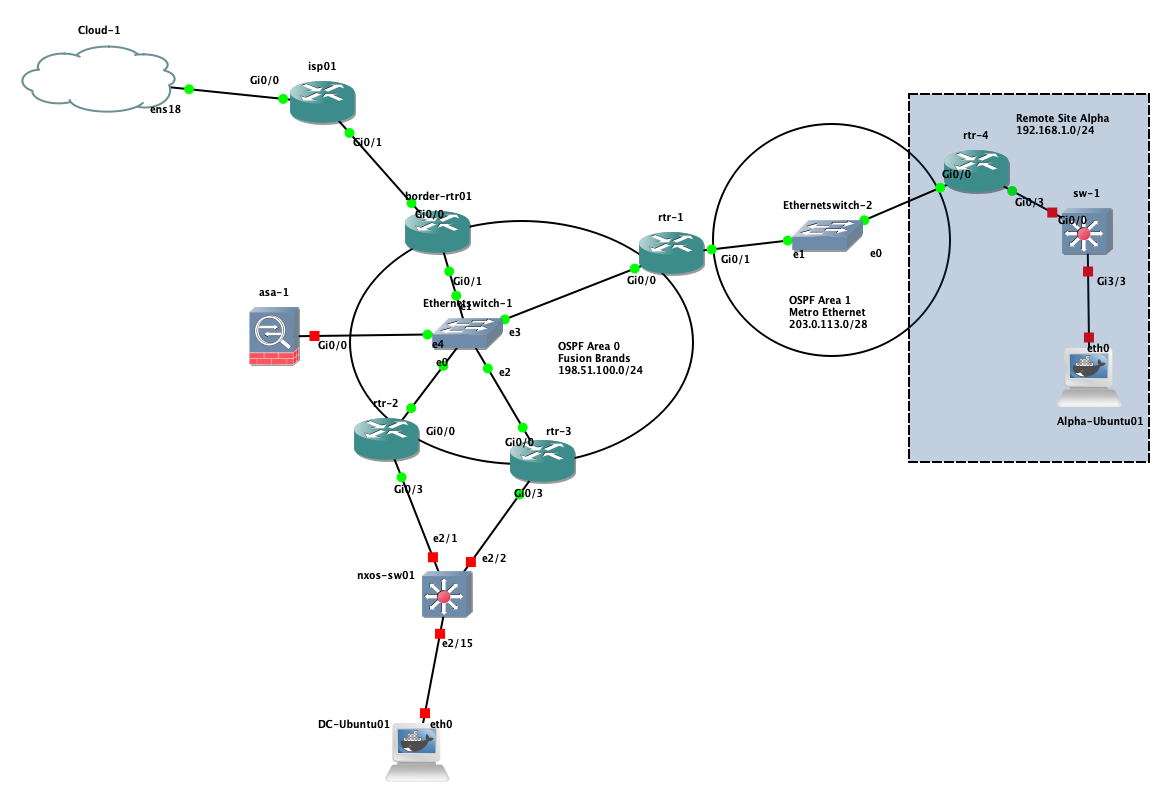
\includegraphics[width=\textwidth]{assets/base_setup.png}
\end{frame}

\begin{frame}
  \frametitle{Ansible Network Modules}
  \begin{block}{Ansible Network Modules}
    The whole list of Network modules and their corresponding requirements
    can be found with your favorite search engine on term of "Ansible Network Modules" 
    - which will take you to this link: \url{https://docs.ansible.com/ansible/latest/modules/list_of_network_modules.html}
    This will be included on the notes for this.
    \end{block}
\end{frame}

\begin{frame}
  \frametitle{Ansible Network Modules Page}
    Let's take a look at those modules
\end{frame}


\begin{frame}
  \frametitle{Summary}
    To review what we accomplished today:
    \begin{itemize}
      \item <1-> Reviewed the lab environment that will be leveraged in the next module
      \item <2-> Detailed where to get more information about network modules on the Ansible documentation pages
    \end{itemize}
\end{frame}

\begin{frame}
  \frametitle{Contact}
  \huge
  You can find me and more contacts on the Packet Pushers Slack Channel. 
  \linebreak
  \begin{center}
    \normalsize
    \faSlack \hspace{.1cm}jvanderaa  
  \end{center}
  
\end{frame}

\end{document}